\chapter{System Architecture and Methodology}
\label{chap:system_architecture_methodology}

% Overview of the DQN-based system design integrating SUMO simulation with reinforcement learning
\section{System Architecture}
\label{sec:system_architecture}

The system uses a Deep Q-Network controller with SUMO as the traffic environment. During design, the control action was kept close to what a traffic signal can realistically do: at a fixed decision interval, the controller can either hold the current phase or move to the next phase in the cycle. This avoids an unnecessarily large action space while still allowing the agent to respond to changing queue conditions at Thapathali T1.

At each 15-second step, the state representation module reads lane-level
values through SUMO's TraCI interface. The 21-dimensional state vector
contains four parts:

\begin{itemize}
    \item PCU-weighted vehicle load on 7 origin lanes,
    \item maximum waiting time on 6 stopline lanes,
    \item PCU-weighted vehicle load on 5 outgoing lanes,
    \item a 3-dimensional one-hot encoding of the active signal phase.
\end{itemize}

This combination was used because vehicle count alone would not separate
light vehicles from heavier vehicles, and queue length alone would not
show whether downstream discharge was blocked.

The DQN uses two neural networks with the same structure. The online Q-network receives the 21-dimensional state and passes it through three fully connected hidden layers of 128, 64, and 32 neurons using ReLU activation. Its output contains two Q-values, one for STAY and one for NEXT. The target network is updated less frequently by copying the online network weights, which makes the learning target more stable during training.

A replay buffer stores up to 10,000 past experience tuples: state, action, reward, next state, and the episode termination flag. During training, a random mini-batch of 64 transitions is sampled for the Q-learning update. This breaks the direct ordering of consecutive simulation steps, which is important because traffic states at adjacent seconds are highly correlated. Without replay, the network would mostly learn from the most recent traffic pattern instead of from the wider range of situations seen across the 300 training episodes.

An $\epsilon$-greedy strategy controls exploration. In the early episodes, the agent selects random actions often enough to populate the replay buffer with different queue and phase conditions. As $\epsilon$ decays after each episode, the controller gradually shifts toward the actions suggested by its learned Q-values. A small amount of exploration remains near the end of training so that the policy does not become fixed too early around a weak phase-selection pattern.

The action space consists of 2 discrete actions - STAY and NEXT - applied over a cyclic sequence of 3 predefined signal phases. At each 15-second decision interval the agent either maintains the current active phase to continue serving the same traffic direction or advances to the next phase in the cycle to serve a different approach. Each phase transition includes a 3-second yellow interval to preserve realistic signal behaviour in the simulation.

\begin{figure}[H]
    \centering
    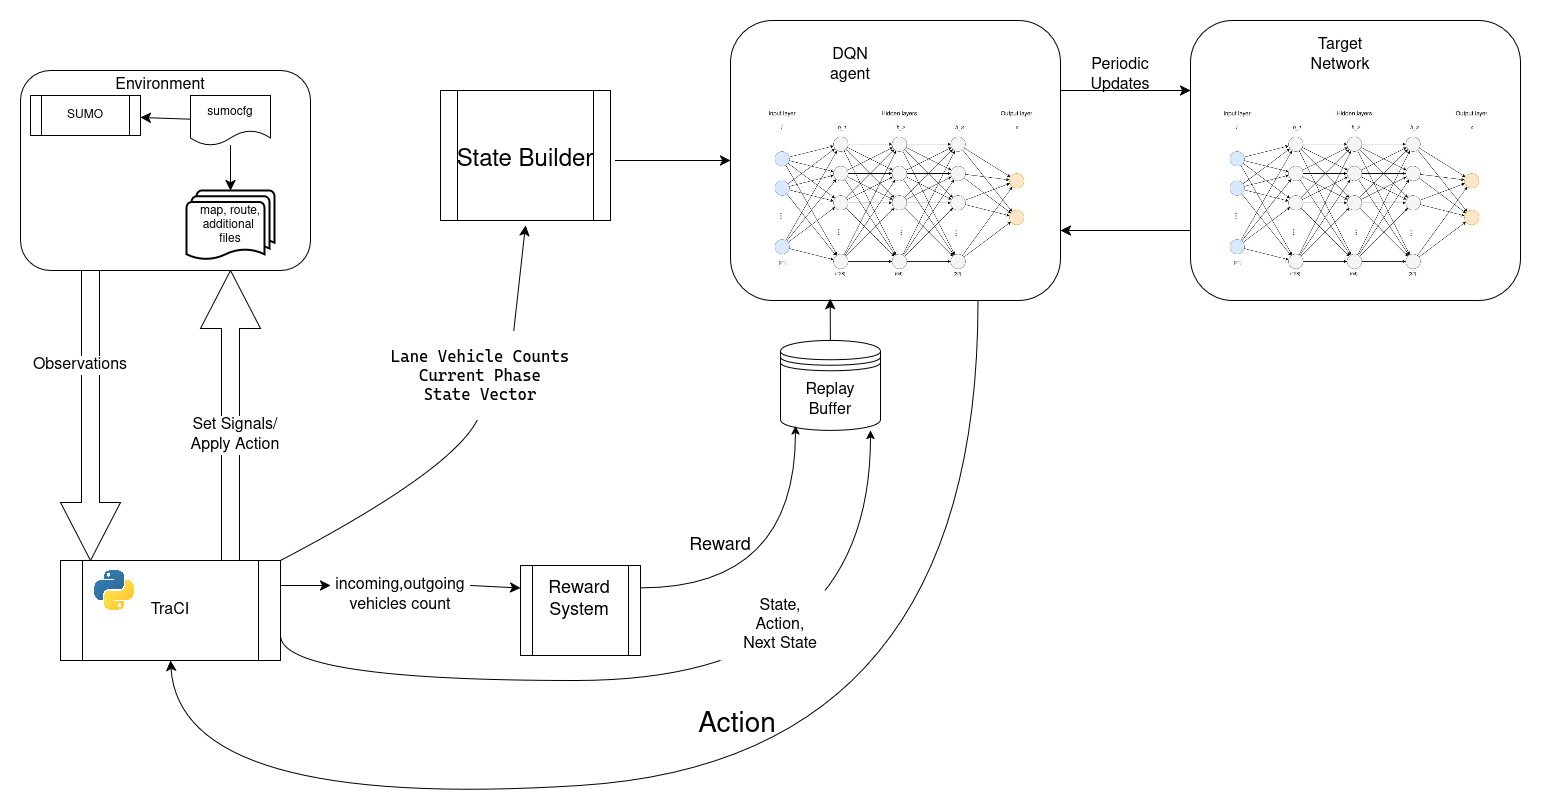
\includegraphics[width=\textwidth]{src/images/figures/system_diagram.jpeg} 
    \caption{Block Diagram of DQN-Based Traffic Signal Control System}
    \label{fig:system_block_diagram}
\end{figure}


\section{Use Case Diagram}
\label{sec:use_case_diagram}

Figure \ref{fig:use_case_diagram} shows how the simulation workflow is
split between four actors: the Traffic Engineer, Evaluation Analyst, SUMO
Simulator, and DQN Agent. The Traffic Engineer prepares the scenario,
loads the trained model, and starts the simulation. The DQN Agent then
observes the state, selects STAY or NEXT, applies the signal phase, and
stores the transition for training.

The Evaluation Analyst role is separated because evaluation must run the
DQN policy and the fixed timer on the same demand. The SUMO Simulator
acts as the environment for both training and testing, so the controller
comparison is not affected by changing the traffic input.

\begin{figure}[H]
    \centering
    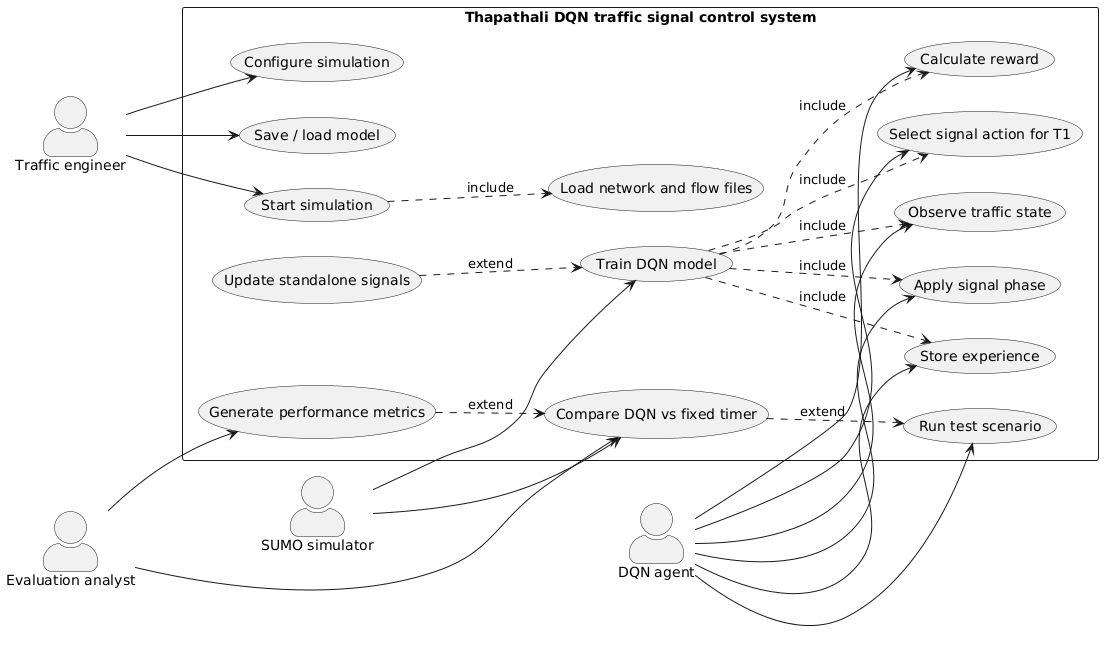
\includegraphics[width=\textwidth]{src/images/figures/USECASE_REPORT.png}
    \caption{Use case diagram of the Thapathali DQN traffic signal control system}
    \label{fig:use_case_diagram}
\end{figure}

\section{Class Diagram}
\label{sec:class_diagram}

Figure \ref{fig:class_diagram} shows the main code structure. TrainDQN is
the entry point for training. It creates the SumoEnvironment and passes
control to the DQNAgent. SumoEnvironment handles TraCI communication,
including state extraction, reward calculation, phase control, and metric
collection.

DQNAgent contains the learning logic. It uses two DQNetwork instances:
one online network for action selection and one target network for stable
targets. ReplayBuffer stores transitions for experience replay. The
configuration class keeps lane names, phase definitions, file paths, and
hyperparameters in one place. FixedTimerController is kept separate so it
can be used as a baseline during evaluation.

\begin{figure}[H]
    \centering
    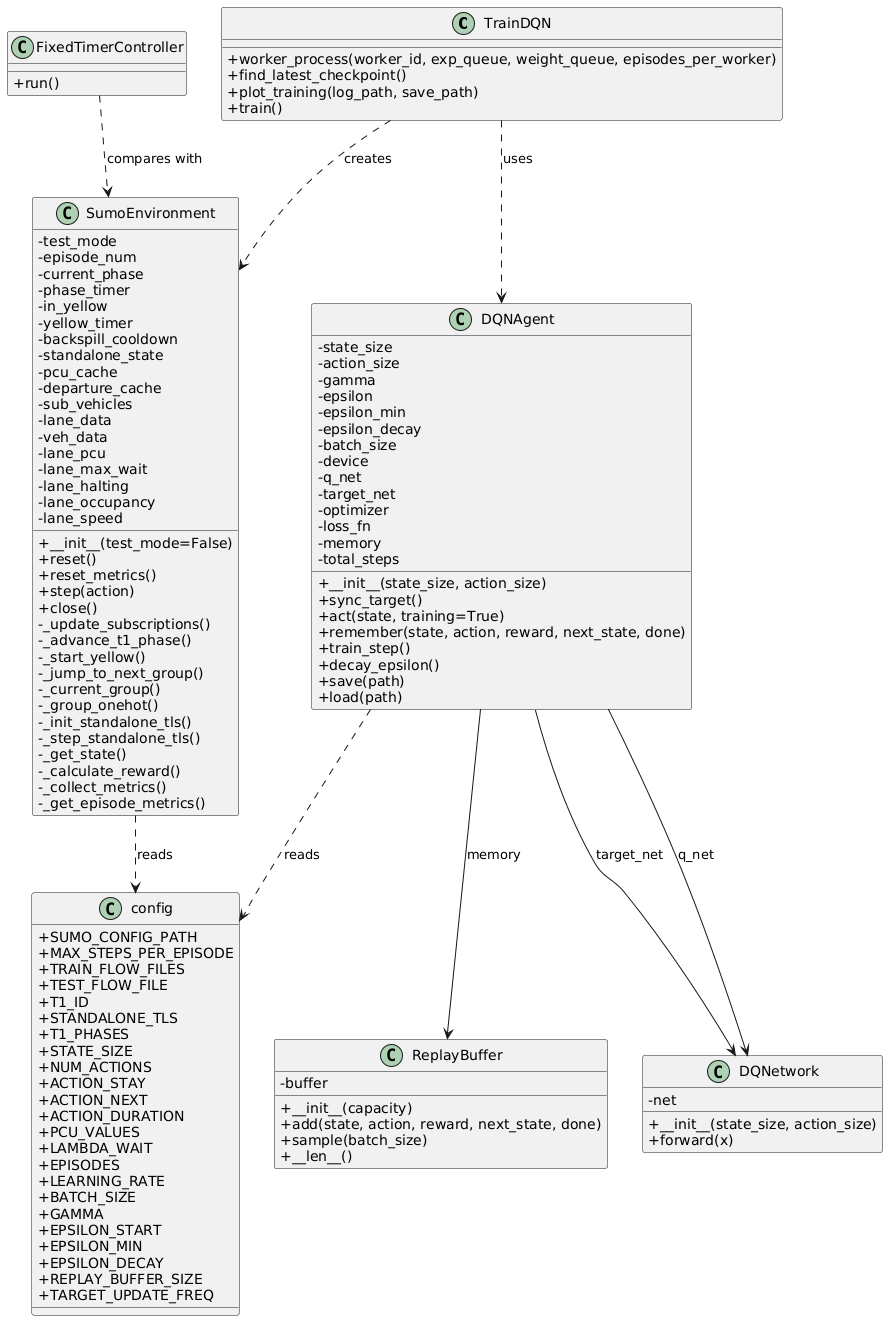
\includegraphics[width=\textwidth]{src/images/figures/Class_Diagram.png}
    \caption{Class diagram of the Thapathali DQN traffic signal control system}
    \label{fig:class_diagram}
\end{figure}

\section{Sequence Diagram}
\label{sec:sequence_diagram}

Figure \ref{fig:sequence_diagram} gives the order of operations from
training to evaluation. The process begins with train(), which creates
the DQNAgent and SumoEnvironment. SUMO then loads the road network and
vehicle-flow files.

Each training episode starts with a reset. At every decision step, the
agent observes the state, chooses STAY or NEXT, and applies the phase for
15 seconds. If NEXT is selected, a 3-second yellow transition is inserted
before the next phase. The environment returns the reward and next state,
and the agent stores the transition before training on replay samples.

Evaluation uses the same test scenario twice: first with
FixedTimerController and then with the saved DQN model. The two metric
sets are compared after both runs finish.

\begin{figure}[H]
    \centering
    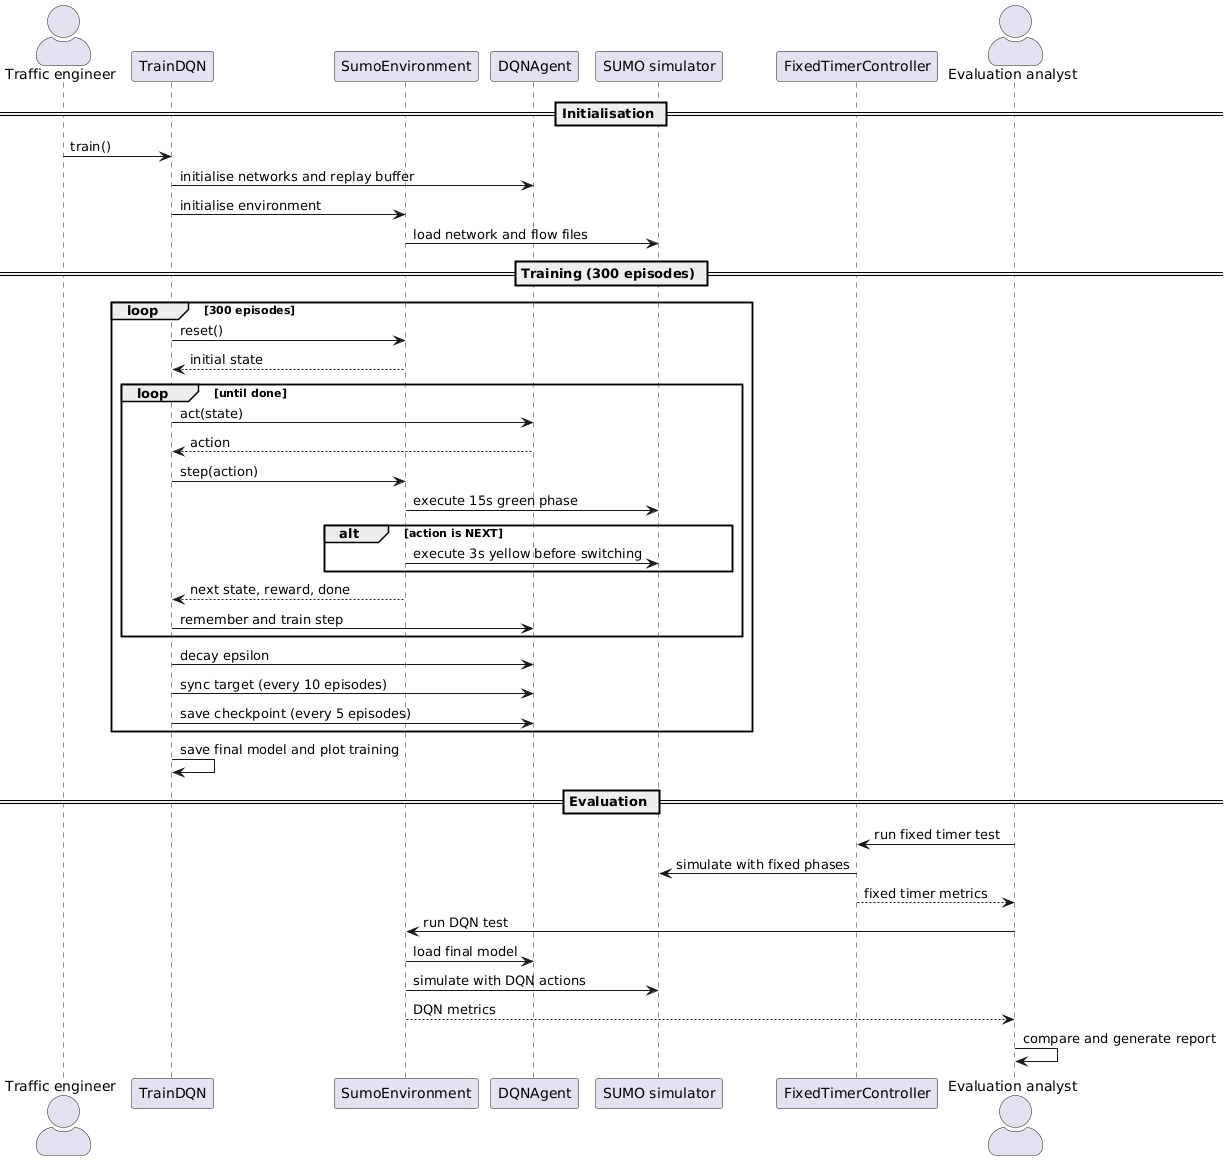
\includegraphics[width=\textwidth]{src/images/figures/Sequence_diagram.png}
    \caption{Sequence diagram of the Thapathali DQN traffic signal control system}
    \label{fig:sequence_diagram}
\end{figure}

% Data sources and field survey methodology used to ground the simulation in real traffic patterns
\section{Data Analysis}
\label{sec:data_analysis}

\subsection{Data Collection}
\label{subsec:data_collection}
Primary traffic-flow data for the network model was taken from \textit{A Case Study of Thapathali Intersection} by Lav Maharjan \cite{maharjan2023performance}. The source study provides five days of observations, covering three weekdays and two weekend days from 6:00 AM to 10:15 PM. This was sufficient for the scope of the project because it includes both peak periods and lower-demand transition hours, although it does not cover unusual events such as road closures, festivals, or accidents.

The available data was represented using \gls{pcu} \gls{od} values and
vehicle counts. The \gls{pcu} \gls{od} data was available for one morning
peak interval and one evening peak interval. Vehicle counts, however,
were available across smaller time intervals.

Because OD proportions were not available for every interval, the
implementation interpolates between the observed AM and PM patterns and
then allocates vehicle counts by class. This is an approximation, but it
keeps the generated demand tied to measured Thapathali data rather than
using arbitrary synthetic flows.

\subsection{Data Representation}
\label{subsec:data_representation}
\begin{table}[H]
    \centering
    \small
    \caption{Vehicle Class and Adopted PCU Factors}
    \label{tab:pcu_factors}
    \begin{tabular}{p{7cm}p{3cm}c}
        \toprule
        \textbf{Vehicle Class} & \textbf{Representation} & \textbf{Adopted PCU Factor} \\
        \midrule
        Light Vehicle & LV & 1.5 \\
        Heavy Vehicle & HV & 3 \\
        Bus & B & 3 \\
        Mini Bus & MB & 2.5 \\
        Micro Bus & MIB & 1.5 \\
        Car & C & 1 \\
        Four-Wheel & F & 1 \\
        Tempo & T & 0.75 \\
        Utility & U & 0.75 \\
        Two-Wheeler & TW & 0.25 \\
        \bottomrule
    \end{tabular}
\end{table}

\subsection{OD Data Allocation}
\label{subsec:od_allocation}
Vehicle allocation was handled with a Python script using \texttt{pandas}, \texttt{numpy}, and \texttt{matplotlib}. The script was needed because the available traffic data did not directly provide a complete SUMO route file; vehicle counts had to be distributed across OD pairs and vehicle classes before simulation.

The primary input data consists of:
\begin{itemize}
    \item \textbf{Vehicle Count Data (\texttt{vehicle\_count.xlsx}):} Contains the number of vehicles for various vehicle classes during 15-minute intervals.
    \item \textbf{PCU OD Data (\texttt{pcu\_od.xlsx}):} Provides the proportions of \gls{pcu} allocated to each \gls{od} pair for AM and PM periods.
\end{itemize}

\subsubsection{Data Cleaning}
\begin{itemize}
    \item Non-numeric characters are removed from vehicle count and \gls{pcu} data.
    \item Invalid data is replaced with zero.
    \item Data is converted to numeric format for proper calculation and allocation.
    \item Vehicles with low counts were grouped into similar vehicle types.
    \item Vehicles with same \gls{pcu} and sizes were grouped into one vehicle type.
\end{itemize}

\subsubsection{Vehicle Allocation Process}
For each vehicle class and \gls{od} pair, the following process is followed:
\begin{itemize}
    \item \textbf{Proportions Calculation:} AM and PM proportions are calculated based on the \gls{pcu} data.
    \item \textbf{Allocation via Largest Remainder Method:} Vehicles are initially allocated proportionally, and leftover vehicles are distributed to ODs with the largest fractional values.
    \item \textbf{Piecewise Interpolation:} For each 15-minute interval, vehicle proportions are dynamically interpolated using piecewise interpolation.
\end{itemize}

\subsubsection{Maternity Restrictions}
For certain ODs related to maternity, only specific vehicle classes are allowed (\eg cars, two-wheelers, four-wheel vehicles, and utility vehicles), based on real-world traffic constraints.

\subsubsection{Output Generation}
The final allocated vehicle counts are saved to Excel files, including:
\begin{itemize}
    \item 15-minute interval counts for every \gls{od} and vehicle class.
    \item A summary sheet showing total vehicles and AM/PM proportions.
    \item A verification sheet ensuring correct and consistent allocation.
\end{itemize}

\section{Environment Setup for Traffic Simulation}
\label{sec:env_setup}

The SUMO environment was prepared by editing the Thapathali road network in NETEDIT. The network was saved as \texttt{map.net.xml}, which stores the junctions, road edges, lane connections, and traffic-signal logic used by the simulator. This step matters because small errors in lane connections or phase definitions can produce unrealistic queues before the DQN agent is even introduced.

After the network was prepared, vehicle movement was defined through \texttt{routes.rou.xml}. This file specifies each route, departure pattern, vehicle type, and flow. The generated flows allow vehicles to enter the network across the simulation period rather than appearing as a single batch, which gives the controller a changing traffic state to respond to.

The \texttt{vtypes.xml} file defines various vehicle types used in the simulation, each with specific attributes such as length, maximum speed, acceleration, and deceleration. These characteristics are essential for accurately simulating vehicle behavior across different classes.

The \texttt{flows.xml} file captures vehicle flow data and traffic signal phases. This file defines how many vehicles pass through each edge of the network in specific time intervals and the corresponding traffic signal phases.

The Python controller interacts with SUMO through \gls{traci}. Through this interface, the script reads lane-level vehicle counts and waiting times, applies signal actions, and records the metrics used for evaluation. This is the link that turns the SUMO network from a passive simulation into an environment for reinforcement learning.

\begin{figure}[H]
    \centering
    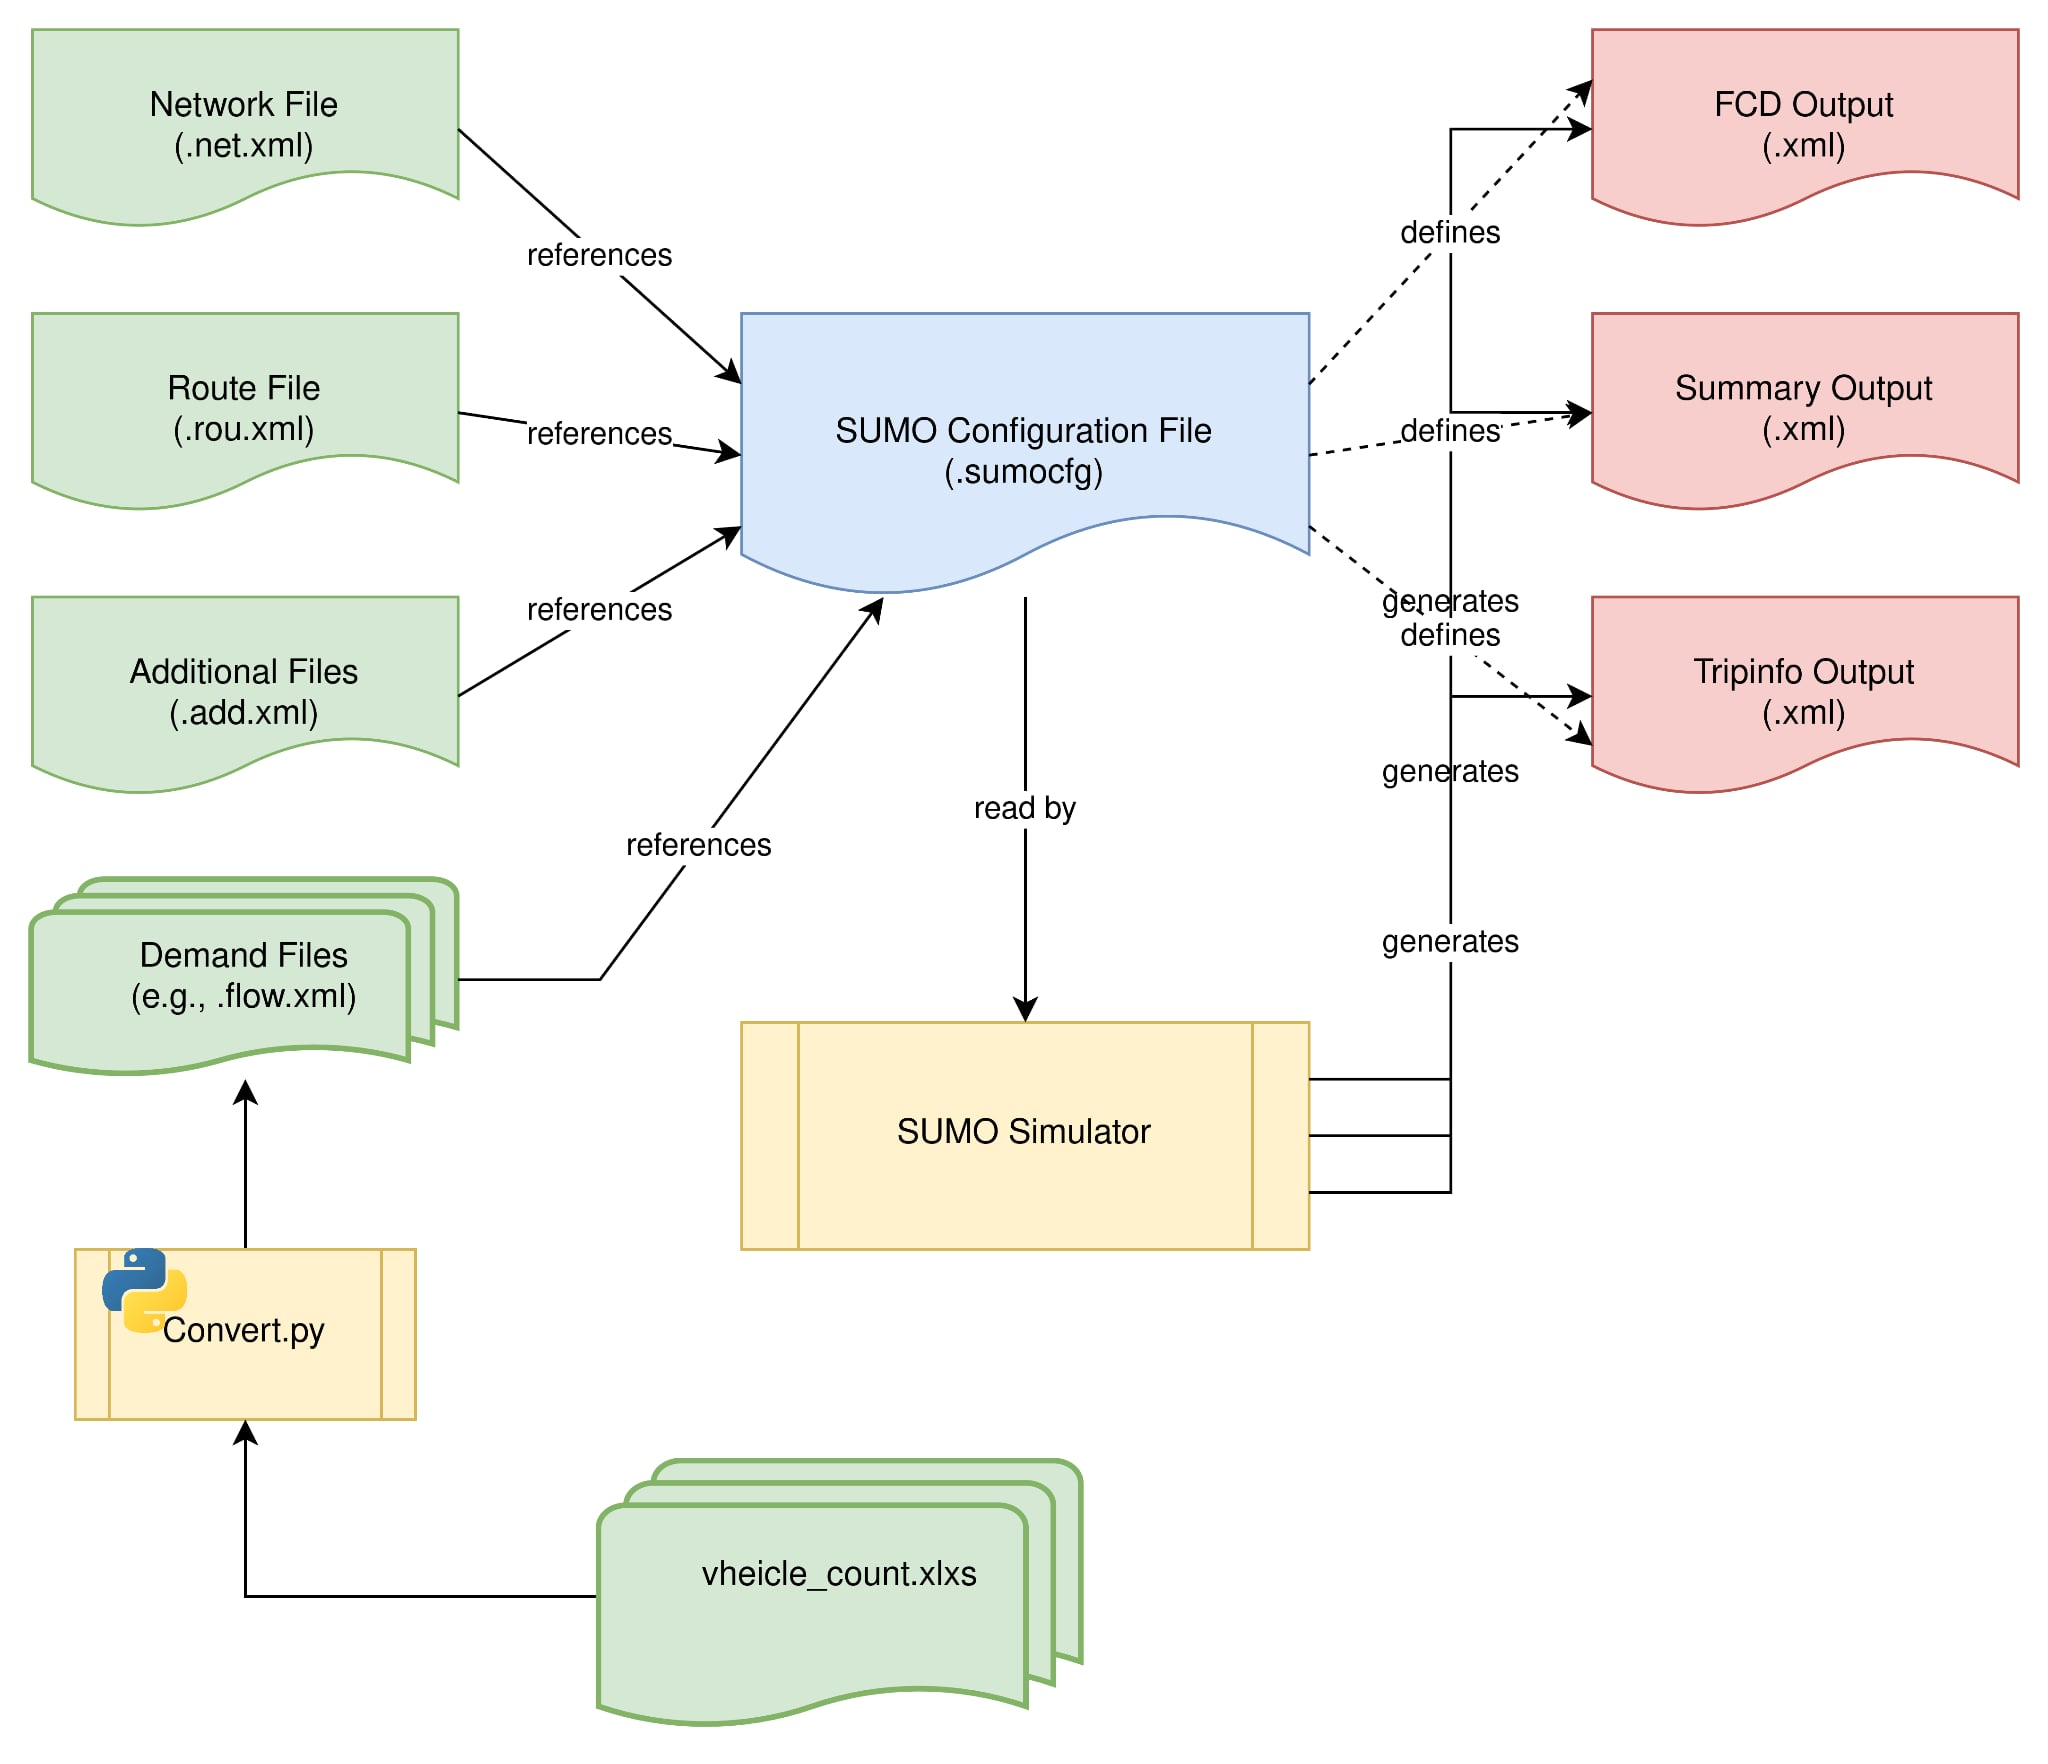
\includegraphics[width=\textwidth]{src/images/figures/sumoenviroment.jpeg}
    \caption{SUMO Environment Block Diagram}
    \label{fig:sumo_env_diagram}
\end{figure}

% Design of the DQN agent including state vector, action space, reward shaping, and network layers
\section{DQN Agent Development}
\label{sec:dqn_development}

\subsection{State Representation}
The \gls{dqn} agent observed key traffic conditions at each 15-second decision step, including PCU-weighted vehicle loads on incoming and outgoing lanes, maximum waiting times at stopline lanes, and the current active signal phase. These parameters were combined into a fixed-length 21-dimensional state vector representing the intersection status at each decision step.


\[
s_t = \bigl[ 
  \underbrace{p_1, p_2, \dots, p_7}_{\text{Incoming PCU (7)}}, \;
  \underbrace{w_1, w_2, \dots, w_6}_{\text{Stopline Max Wait (6)}}, \;
  \underbrace{p_{o1}, p_{o2}, \dots, p_{o5}}_{\text{Outgoing PCU (5)}}, \;
  \underbrace{0, 1, 0}_{\text{Current Phase (3)}}
\bigr]
\]


\subsection{Action Space}

The traffic signal at Thapathali T1 operates across three predefined phases (P1, P2, P3) in a cyclic sequence. At every 15-second decision interval the DQN agent selects one of two actions - Action 1 (STAY) or Action 2 (NEXT) - to control the signal timing. A phase can be held for a maximum of 60 seconds (4 consecutive STAY actions) before automatically advancing to the next phase, ensuring no traffic direction is starved indefinitely.
\begin{itemize}
  \item \textbf{Action 1 (STAY)}: 
The agent maintains the current active phase for another 15 seconds, allowing continued service to the same direction.
  \item \textbf{Action 2 (NEXT)}: The agent advances to the next phase in the cycle, switching service to the next direction. Each phase transition includes a 3-second yellow interval to ensure realistic and safe signal timing.
\end{itemize}

\subsection{Reward Function}
\noindent The reward function was based on Max-Pressure theory. Pressure was calculated from the difference between stopline PCU accumulation and outgoing PCU discharge:

\begin{equation}
R = -\left(\sum_{l \in L_{\text{stop}}} \text{PCU}(l) - \sum_{l \in L_{\text{out}}} \text{PCU}(l)\right) - \lambda \sum_{l \in L_{\text{stop}}} \sum_{v \in l} \text{PCU}(v) \cdot w^{acc}(v)
\end{equation}

\textbf{Where:}
\begin{itemize}
    \item $L_{\text{stop}}$ - set of 6 stopline lanes
    \item $L_{\text{out}}$ - set of 5 outgoing lanes
    \item $\mathrm{PCU}(l)$ - total PCU-weighted vehicle load on lane $l$ at current step
    \item $\mathrm{PCU}(v)$ - PCU value of individual vehicle $v$
    \item $w^{\text{acc}}(v)$ - accumulated waiting time (seconds) of vehicle $v$ since simulation start
    \item $\lambda = 0.0004$ - weighting factor balancing throughput and wait time penalty
\end{itemize}


\section{Design Justification}
\label{sec:design_justification}

The reward design was revised several times during implementation. A pure
delay penalty was the first simple option, but accumulated waiting time
keeps increasing inside an episode. In early tests, that made the target
values too large and the loss unstable.

A throughput-only reward was also considered, but it was not suitable for
Thapathali. Some outgoing links clear vehicles more easily because of
their width and geometry. A reward based only on discharge could
therefore favour an easier outgoing path rather than the approach with
the more urgent queue.

The adopted reward therefore uses Max-Pressure as the main signal and
adds a smaller waiting-time penalty. The pressure term compares stopline
PCU with outgoing PCU, which matches the actual control question: is the
selected phase helping vehicles leave the intersection? The waiting-time
term, scaled by $\lambda = 0.0004$, was added to prevent the controller
from repeatedly ignoring a low-volume approach. In this formulation,
fairness acts as a correction to the pressure objective, not as a
replacement for it.

\subsection{Impact on Learning}
\label{subsec:impact_on_learning}

The reward is used at every Q-learning update, so it had to be easy for
the agent to interpret. When a phase clears vehicles, outgoing PCU rises
and stopline PCU falls; the reward becomes less negative. When the
controller keeps an unhelpful phase, the opposite happens and the reward
worsens. This gives the network a direct signal linking the phase choice
to the observed traffic response.

The accumulated wait penalty handles a case that pressure alone can miss.
If a small approach keeps waiting while the larger approaches dominate
the pressure term, the penalty gradually makes that delay visible to the
agent. This reduces the chance of learning a policy that looks efficient
in aggregate but is unacceptable for one movement.

Together, the two terms connect training with the evaluation metrics used
later in the report. The pressure term is related to discharge and
throughput efficiency, while the waiting-time term is related to delay.
The reward is therefore not an arbitrary score; it represents the same
trade-off measured in the results chapter.

\subsection{Neural Network Architecture}

The agent uses a feed-forward neural network. The input layer accepts the
21-dimensional state vector. Three hidden layers with 128, 64, and 32
neurons use ReLU activation. The output layer produces two Q-values,
corresponding to STAY and NEXT. During exploitation, the agent selects
the action with the higher estimated value.

Two identical networks were used: a Q-network for action selection and a target network to stabilise learning during training. The target network weights were updated every 10 episodes by copying the Q-network weights, preventing oscillations and divergence during the training process.
\begin{figure}[H]
    \centering
    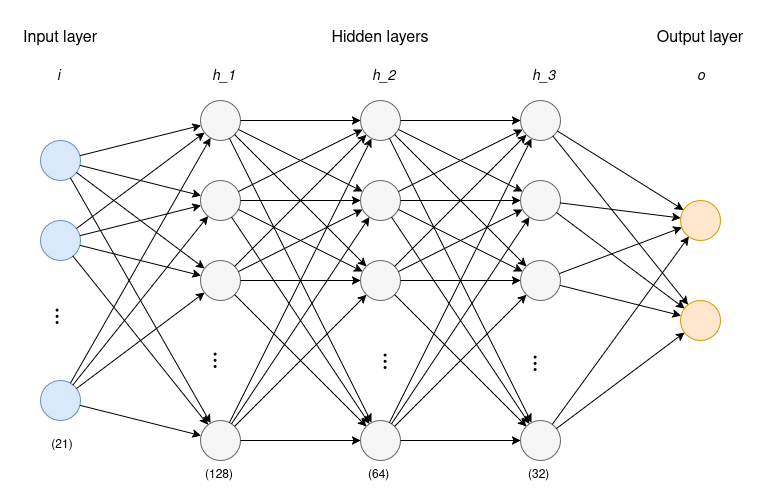
\includegraphics[width=0.85\textwidth]{src/images/figures/NN.png}
    \caption{Neural Network Architecture for Q-value Prediction}
    \label{fig:nn_architecture}
\end{figure}



\section{Hyperparameter Selection and Sensitivity}

The DQN agent depends on several hyperparameters. The values below were
chosen from standard DQN practice and then checked against the practical
limits of this simulation: 300 training episodes, a single intersection,
and CPU-friendly training time.

\subsection{State Dimensionality (21 dimensions)}

The 21-dimensional state vector was kept small enough to train reliably
but large enough to describe the intersection. Origin-lane PCU values
show where demand is building. Stopline waiting times show whether one
approach has waited too long. Outgoing-lane PCU values indicate whether
vehicles are actually discharging downstream. The phase encoding is also
necessary; without it, the same queue pattern could mean different
things depending on which phase is currently active.

\subsection{Replay Buffer Capacity (10,000 transitions)}

The replay buffer stores past transitions so that training batches are
not made only from consecutive simulation steps. A very small buffer made
the agent depend too much on recent traffic conditions. A much larger
buffer would add diversity, but it would also take more episodes to fill
and use properly. With 10,000 transitions and a 15-second decision step,
the buffer covers roughly 41 simulated hours, which is enough to mix
different demand periods without making training unnecessarily heavy.

\subsection{Batch Size (64 transitions)}

The batch size was set to 64 transitions. Smaller batches produced
noisier updates, while larger batches increased the cost of each training
step. A batch of 64 gave a useful mix of stored experiences while keeping
the training loop practical on the available hardware.

\subsection{Discount Factor \( \gamma = 0.95 \)}

The discount factor controls how far ahead the agent looks. A value close
to zero would make the controller react only to the next 15-second step.
A value of 1.0 would give too much weight to far-future rewards, where
the effect of one signal decision is harder to isolate.

At \( \gamma = 0.95 \), a reward five decision steps later, or 75 seconds
ahead, still keeps about 77\% of its value. That horizon is long enough
to capture a queue-clearing decision without making the learning target
too diffuse.

\subsection{Epsilon Start (\( \varepsilon = 1.0 \)), Minimum (\( \varepsilon_{\min} = 0.01 \)), and Decay (\( \varepsilon_{\text{decay}} = 0.985 \))}

The exploration schedule starts with \( \varepsilon = 1.0 \), so the
early policy is deliberately random. This prevents the untrained network
from committing too early to whichever action initially receives a higher
Q-value.

With a decay factor of 0.985, exploration falls to about 0.18 by episode
100 and reaches 0.01 near episode 300. Faster decay would make the agent
exploit too early. Slower decay would spend too much of the limited
training budget on random actions.

\subsection{Target Network Update Frequency (every 10 episodes)}

The target network was updated every 10 episodes. Updating it at every
step would make the target move with the online network and increase the
risk of unstable Q-values. Updating it very rarely would leave the agent
learning from stale targets, especially early in training. Ten episodes
was used as a compromise between those two cases.

\subsection{Reward Weighting Factor \( \lambda = 0.0004 \)}

The value \( \lambda = 0.0004 \) controls how strongly waiting time
affects the reward. If \( \lambda \) were zero, the controller could
favour high-flow approaches and ignore a smaller queue. If it were much
larger, the agent could become too focused on individual waiting vehicles
and reduce overall discharge. For typical peak-hour stopline loads of
20-30 PCU and accumulated waiting times of 30-60 seconds, the penalty
remains smaller than the pressure term. That keeps waiting time as a
fairness correction rather than the dominant objective.

\subsection{Decision Step Duration (15 seconds)}

The 15-second decision step was chosen after considering switching
overhead. A 5-second step would let the agent react more often, but it
would also create many yellow transitions and reduce useful green time.
A 30-second step would be smoother but less responsive when queues change
quickly. At 15 seconds, the agent can revise its decision four times per
minute while still giving a phase enough time to clear vehicles. The
60-second maximum phase duration prevents one approach from being held
indefinitely.

\subsection{Yellow Phase Duration (3 seconds)}

A 3-second yellow interval is inserted before every phase transition to reflect safe and realistic signal operation. This value is consistent with standard traffic engineering practice for intersection approach speeds in the 25–40 km/h range typical of urban Kathmandu roads. Reducing this to 1–2 seconds would be unsafe; increasing it to 5 seconds would unnecessarily consume green time, particularly at the 15-second decision step resolution where a 5-second yellow would represent one-third of available action time.

\subsection{Hidden Layer Architecture (128 \( \rightarrow \) 64 \( \rightarrow \) 32 neurons)}

The hidden layers were arranged as 128, 64, and 32 neurons. The first
layer gives enough capacity to combine lane loads, waiting times, and
phase indicators. The following layers compress that information before
the final STAY/NEXT decision. A larger network was not used because the
training budget was limited to 300 episodes; increasing capacity without
more data would make memorisation more likely.

\subsection{Learning Rate (\( \alpha = 0.001 \)) for Adam Optimiser}

The Adam learning rate was set to 0.001. This value gave visible learning
progress without the large oscillations observed with overly aggressive
updates in DQN-style training. A much smaller value would likely require
more than 300 episodes to reach a comparable policy.

\subsection{Number of Training Episodes (300)}

The training length was set to 300 episodes because it matches the
epsilon schedule: by that point, exploration has reached its minimum of
0.01. The reward curve in Figure 6-2 also shows the moving average
flattening after roughly episode 250. More episodes could still refine
the policy, but they would mostly do so under near-full exploitation
unless the exploration schedule was changed.




% Training loop covering epsilon-greedy exploration, experience replay, and target network updates
\section{Training Process}
\label{sec:training_process}

\subsection{Learning Strategy}

An $\epsilon$-greedy learning strategy was used during training. The
agent started with $\epsilon = 1.0$, so early decisions were random and
the replay buffer received a wider range of traffic states.

After each episode, $\epsilon$ was multiplied by 0.985. By approximately
episode 300, it reached the minimum value of 0.01. At that point the
agent used the learned policy for almost all decisions while still
retaining a small chance of exploration.
\subsection{Experience Replay}
\noindent Experience replay improved stability by storing transitions in a 10,000-capacity buffer. Random samples were used for training to break temporal correlations.

\subsection{Training Loop}
\noindent The model was trained over 300 episodes. The process included:
\begin{enumerate}
    \item Calculate Target Q: $Q_{\text{target}} = r + \gamma \times \max(Q(s', a'))$.
    \item Calculate Current Q: $Q_{\text{current}} = Q(s, a)$.
    \item Backpropagate Loss: $\text{MSE}(Q_{\text{target}}, Q_{\text{current}})$.
    \item Update policy network weights.
\end{enumerate}

% Pseudocode for the max-pressure reward calculation and the DQN training procedure
\section{Algorithms Used}
\label{sec:algorithms}

\begin{algorithm}
\caption{Reward Calculation}
\begin{algorithmic}[1]
\Require Stopline lane PCU values, Outgoing lane PCU values, Vehicle waiting times
\Ensure Reward value
\Procedure{CalculateReward}{}
    \State $\text{incoming\_pcu} \leftarrow \sum_{l \in L_{\text{stop}}} \text{PCU}(l)$
    \State $\text{outgoing\_pcu} \leftarrow \sum_{l \in L_{\text{out}}} \text{PCU}(l)$
    \State $\text{weighted\_wait} \leftarrow 0$
    \For{all $l \in L_{\text{stop}}$}
        \For{all $v \in l$}
            \State $\text{weighted\_wait} \leftarrow \text{weighted\_wait} + \text{PCU}(v) \cdot w^{acc}(v)$
        \EndFor
    \EndFor
    \State $\text{reward} \leftarrow -(\text{incoming\_pcu} - \text{outgoing\_pcu}) - \lambda \cdot \text{weighted\_wait}$
    \State \Return $\text{reward}$
\EndProcedure
\end{algorithmic}
\end{algorithm}

\begin{algorithm}
\caption{DQN Training Process}
\begin{algorithmic}[1]
\Require Number of episodes $E = 300$, Replay buffer capacity $B = 10000$, 
         Target network update frequency $F = 10$, Batch size $= 64$
\Ensure Trained Q-network
\Procedure{TrainDQN}{$E, B, F$}
    \State Initialize $\epsilon \leftarrow 1.0$, $\epsilon_{min} \leftarrow 0.01$, $\epsilon_{decay} \leftarrow 0.985$
    \State Initialize replay buffer with capacity $B$
    \State Initialize Q-network and target network with random weights
    \For{$episode \leftarrow 1$ to $E$}
        \State Reset environment
        \State $state \leftarrow \text{GetInitialState()}$
        \While{simulation is running}
            \State $action \leftarrow \text{SelectAction}(state, \epsilon)$ \Comment{$\epsilon$-greedy selection}
            \State Execute $action$ for 15 seconds
            \State $reward \leftarrow \text{CalculateReward()}$
            \State $next\_state \leftarrow \text{GetNextState()}$
            \State Store $(state, action, reward, next\_state)$ in replay buffer
            \If{replay buffer has $\geq 64$ samples}
                \State Sample random batch of 64 from replay buffer
                \State Calculate target: $Q_{target} = r + \gamma \times \max_{a'}(Q(s', a'))$
                \State Calculate current: $Q_{current} = Q(s, a)$
                \State Compute loss: $\mathcal{L} = \text{MSE}(Q_{target}, Q_{current})$
                \State Update Q-network weights via backpropagation
            \EndIf
            \State $state \leftarrow next\_state$
        \EndWhile
        \State $\epsilon \leftarrow \max(\epsilon_{min}, \epsilon \times \epsilon_{decay})$ \Comment{Decay exploration rate}
        \If{$episode \mod F = 0$}
            \State Update target network weights from Q-network
        \EndIf
        \If{$episode \mod 5 = 0$}
            \State Save model checkpoint
        \EndIf
    \EndFor
    \State \Return trained Q-network
\EndProcedure
\end{algorithmic}
\end{algorithm}
